\documentclass[a4paper,11pt]{article}

\usepackage[utf8]{inputenc}
\usepackage[T1]{fontenc}
\usepackage[french]{babel}
\usepackage{graphicx}
\usepackage{booktabs}
\usepackage{geometry}
\geometry{margin=2.5cm}
\usepackage{hyperref}
\usepackage{amsmath}
\usepackage{amsfonts}
\usepackage{float}

\title{NET 4103/7431 : Network Science and Graph Learning \\ \large Devoir : Analyse du dataset Facebook100}
\author{Ethan Ducournau}
\date{\today}

\begin{document}

\maketitle

Le code source complet de ce projet, incluant les implémentations des métriques et des modèles GNN, est disponible sur GitHub : \url{https://github.com/e-dcrn/net4103-project}

\section{Introduction \& Question 1 : Lectures}
Ce rapport présente les résultats du travail pratique sur la science des réseaux appliqué au jeu de données \textit{Facebook100}. Ce dataset contient les connexions d'amitié de 100 universités américaines en 2005. L'objectif est d'analyser la topologie de ces réseaux, d'étudier l'assortativité, de prédire des liens et de propager des labels.
Les documents de référence [1, 2, 3] permettent de comprendre l'origine du dataset et les méthodes d'analyse structurelle des réseaux sociaux universitaires.

\section{Question 2 : Analyse des réseaux sociaux avec Facebook100}
L'analyse porte sur la plus grande composante connexe (LCC) de trois universités : Caltech (762 nœuds), MIT (6402 nœuds) et Johns Hopkins (5157 nœuds).

\subsection{(a) Analyse topologique et distributions de degrés}
Les métriques calculées pour chaque réseau sont présentées dans le Tableau \ref{tab:metrics}.

\begin{table}[h]
    \centering
    \caption{Métriques topologiques des réseaux (LCC).}
    \label{tab:metrics}
    \begin{tabular}{lccc}
        \toprule
        \textbf{Réseau} & \textbf{Densité} & \textbf{Clustering Global} & \textbf{Clustering Local Moyen} \\
        \midrule
        Caltech       & 0,05743 & 0,29128 & 0,40912 \\
        MIT           & 0,01226 & 0,18029 & 0,27236 \\
        Johns Hopkins & 0,01403 & 0,19316 & 0,26901 \\
        \bottomrule
    \end{tabular}
\end{table}

\begin{figure}[h]
    \centering
    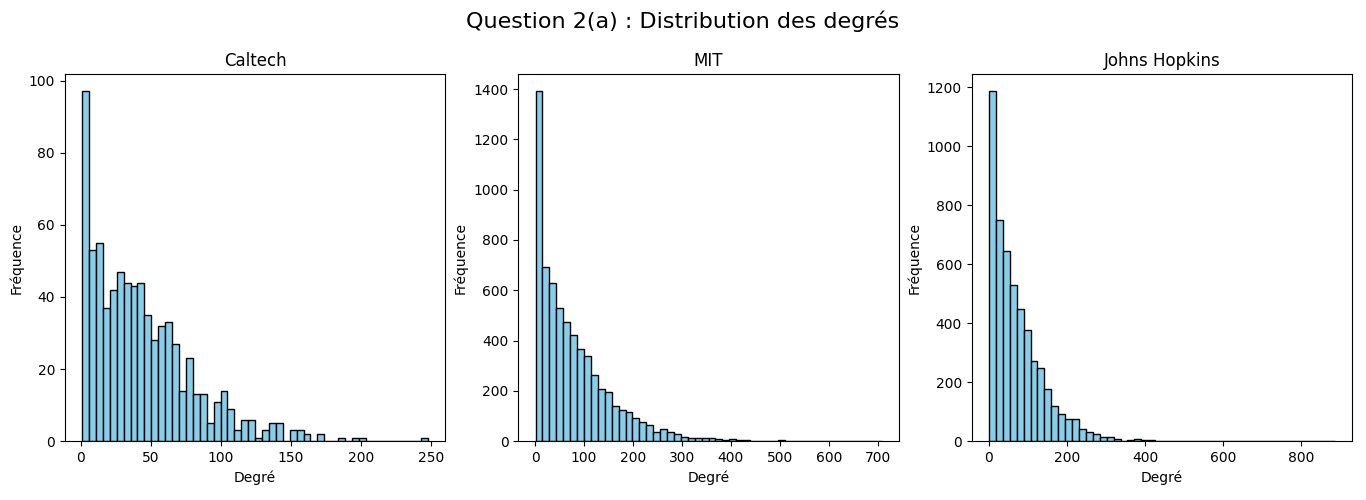
\includegraphics[width=0.9\textwidth]{q2a.png}
    \caption{Distributions des degrés pour Caltech, MIT et Johns Hopkins.}
    \label{fig:q2a}
\end{figure}

\paragraph{Analyse des distributions :}
Comme illustré par la Figure \ref{fig:q2a}, les distributions de degrés montrent que la majorité des étudiants ont un nombre restreint d'amis, tandis qu'un petit nombre d'individus ("hubs") possèdent un degré très élevé. Cette structure est caractéristique des réseaux sociaux réels.

\paragraph{Sparsité et topologie :}
La densité des arêtes pour les trois réseaux est très faible ($< 6\%$), ce qui permet de conclure que ces réseaux sont \textbf{clairssemés} (\textit{sparse}). Cependant, les coefficients de clustering sont très élevés par rapport à la densité, ce qui indique une structure de "petit monde" (\textit{small-world}) avec une forte tendance à la formation de triangles sociaux (fermeture triadique).

\subsection{(b) Corrélation Degré vs Clustering Local}
Le nuage de points de la Figure \ref{fig:q2b} montre la relation entre le degré d'un nœud et son coefficient de clustering local.

\begin{figure}[h]
    \centering
    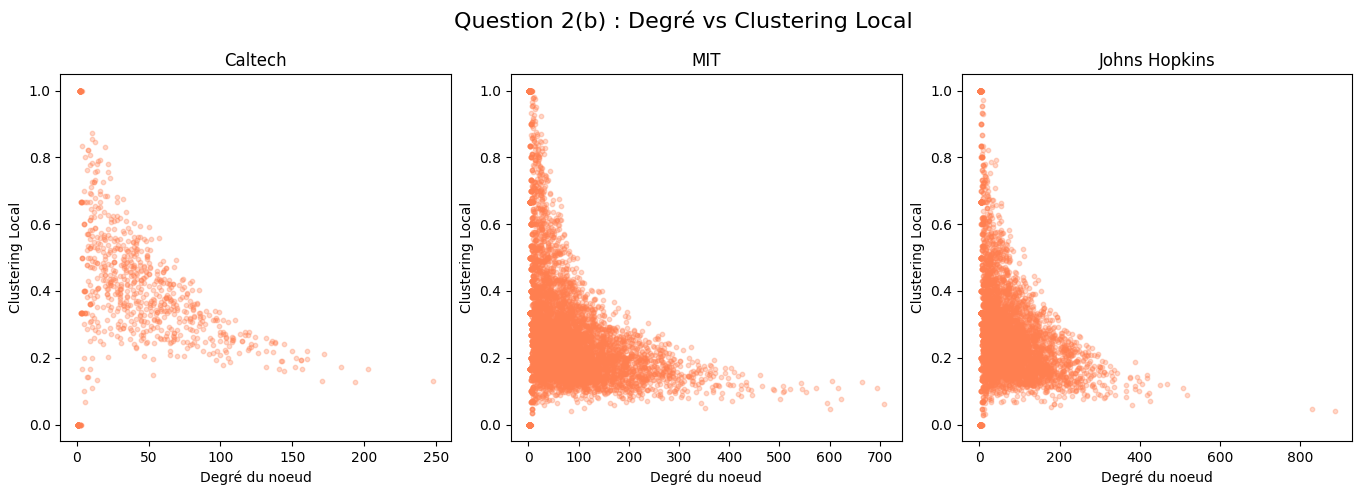
\includegraphics[width=0.9\textwidth]{q2b.png}
    \caption{Degré versus Coefficient de Clustering Local.}
    \label{fig:q2b}
\end{figure}

\paragraph{Observations :}
On observe une tendance générale où les nœuds ayant un faible degré présentent une grande disparité de clustering local, alors que les hubs ont souvent un clustering plus faible. Cela suggère que les individus très connectés servent de ponts entre différentes communautés plutôt que d'être au centre d'un groupe unique ultra-dense.

\paragraph{Similitudes et différences :}
Bien que les échelles varient (Caltech étant plus petit et plus dense), la structure globale de corrélation est similaire entre les trois institutions. Caltech se distingue toutefois par un clustering local moyen nettement plus élevé (0,409), traduisant une cohésion sociale plus forte au sein de cette petite communauté universitaire.

\section{Question 3 : Analyse de l'assortativité sur le dataset Facebook100}

Conformément aux consignes, nous avons traité l'ensemble des réseaux du jeu de données comme des graphes simples et calculé l'assortativité pour cinq attributs : le statut, la spécialité (major), le degré, la résidence (dorm) et le genre. 

Les sections suivantes présentent, pour chaque attribut, un nuage de points de l'assortativité en fonction de la taille du réseau (échelle logarithmique) ainsi que l'histogramme de sa distribution. La ligne pointillée noire indique une assortativité nulle. L'analyse de ces graphiques nous permet de spéculer sur les mécanismes sous-jacents à la formation des amitiés sur Facebook à cette époque.

\subsection{L'homophilie par Statut et Résidence (Forte assortativité)}

\begin{figure}[H]
    \centering
    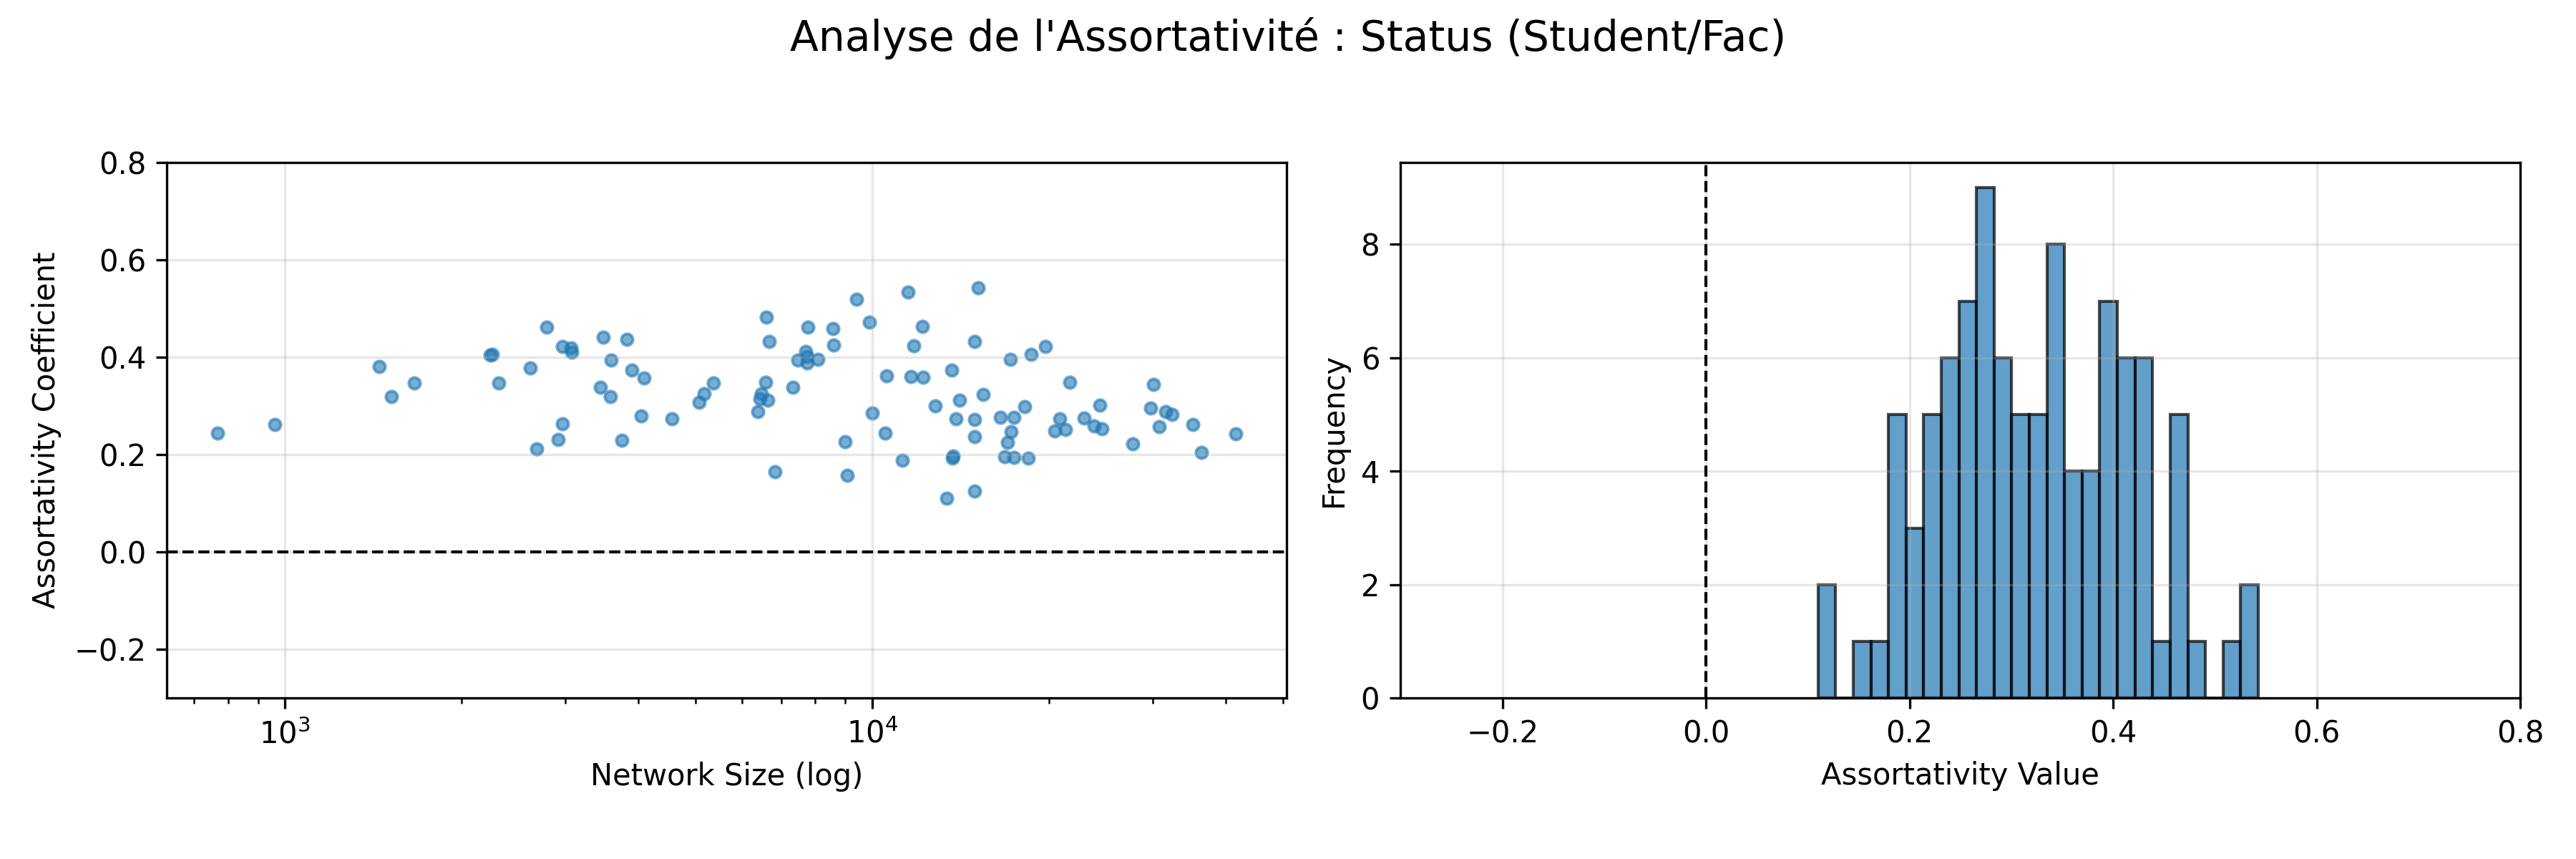
\includegraphics[width=0.9\textwidth]{q3_status.png}
    \caption{Analyse de l'assortativité pour le Statut (Status).}
    \label{fig:q3_status}
\end{figure}

\begin{figure}[H]
    \centering
    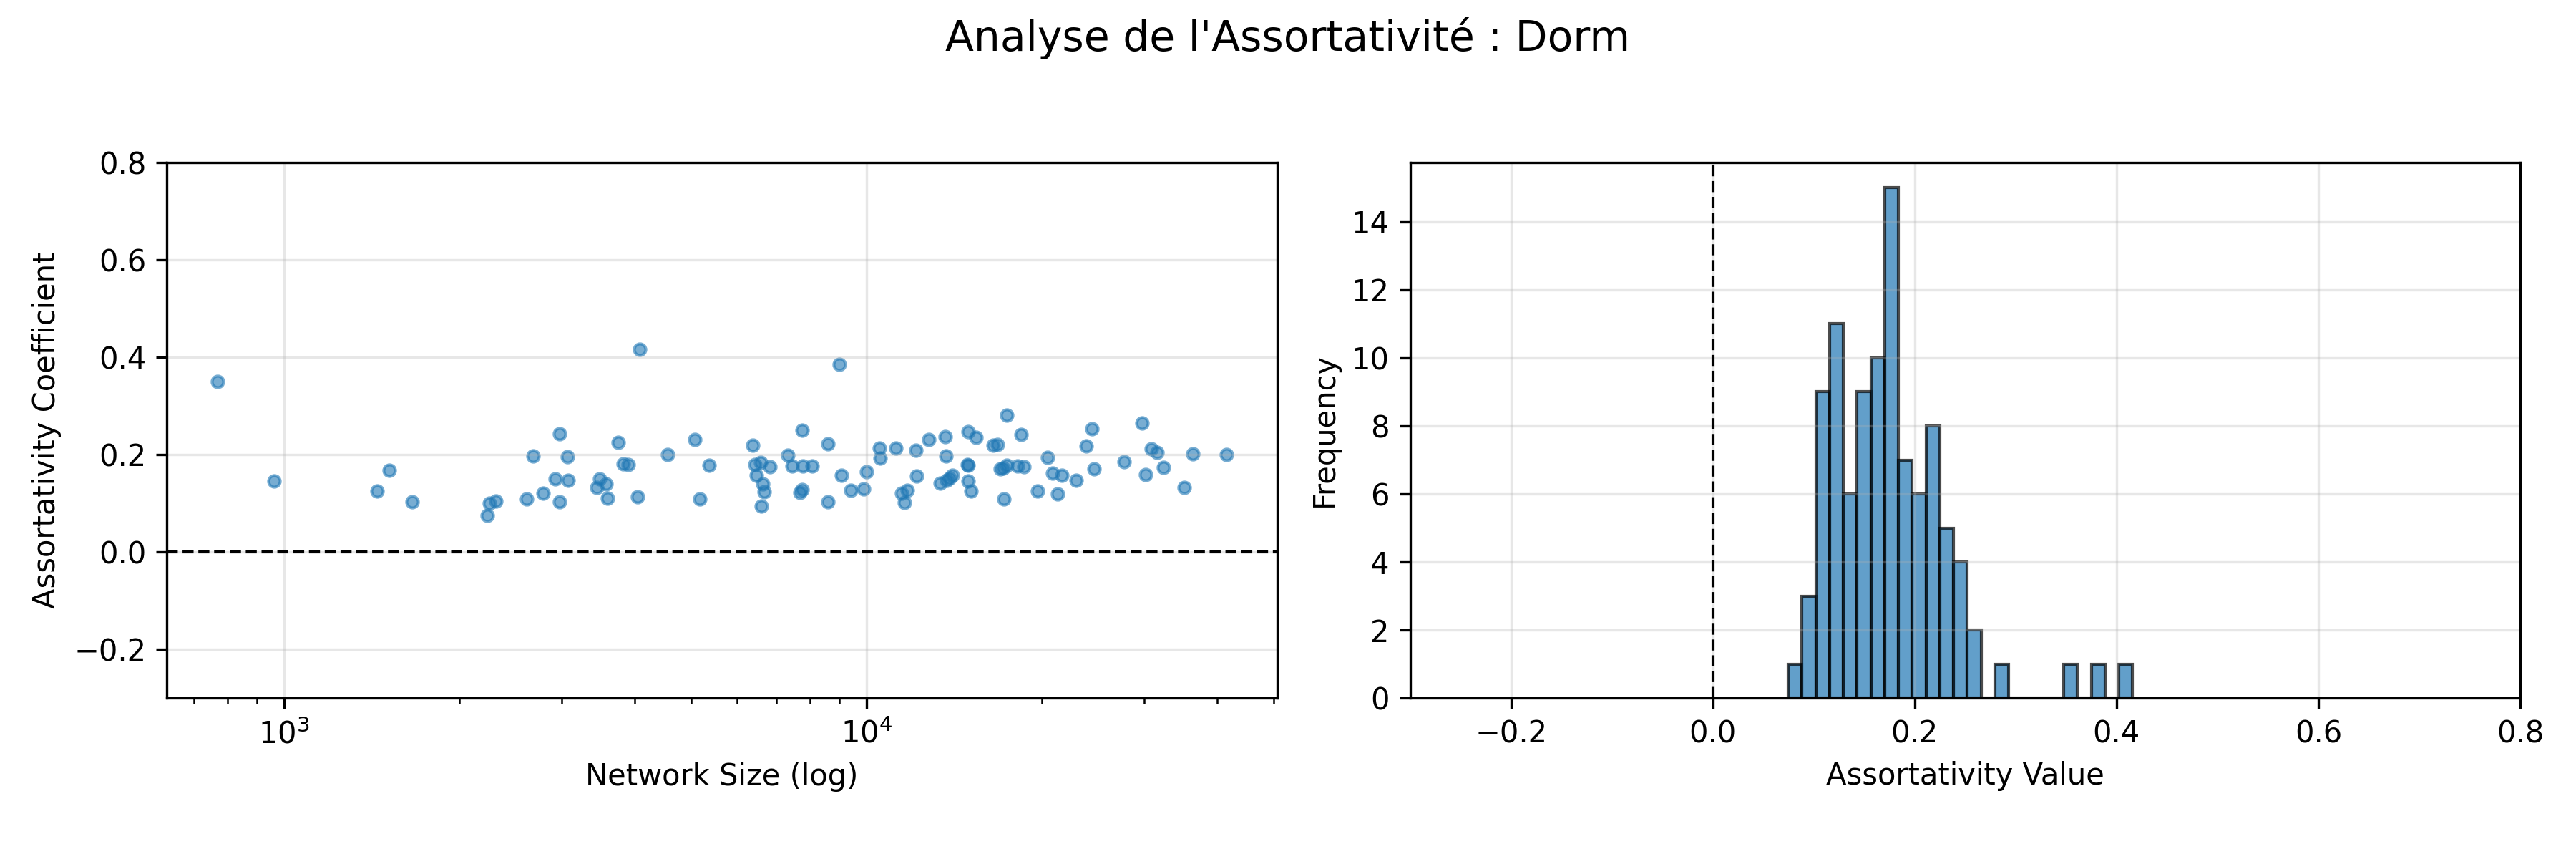
\includegraphics[width=0.9\textwidth]{q3_dorm.png}
    \caption{Analyse de l'assortativité pour la Résidence (Dorm).}
    \label{fig:q3_dorm}
\end{figure}

Les attributs \textbf{Status (Statut)} et \textbf{Dorm (Résidence)} présentent des valeurs nettement positives (majoritairement entre 0,1 et 0,5). Cela traduit une très forte homophilie. La proximité spatiale (partager le même dortoir) et le statut (être étudiant de même cycle) sont des facilitateurs majeurs d'interactions sociales dans la vie réelle, qui se reflètent directement dans la topologie du réseau en ligne.

\subsection{La Spécialité et le Degré (Assortativité modérée à neutre)}

\begin{figure}[H]
    \centering
    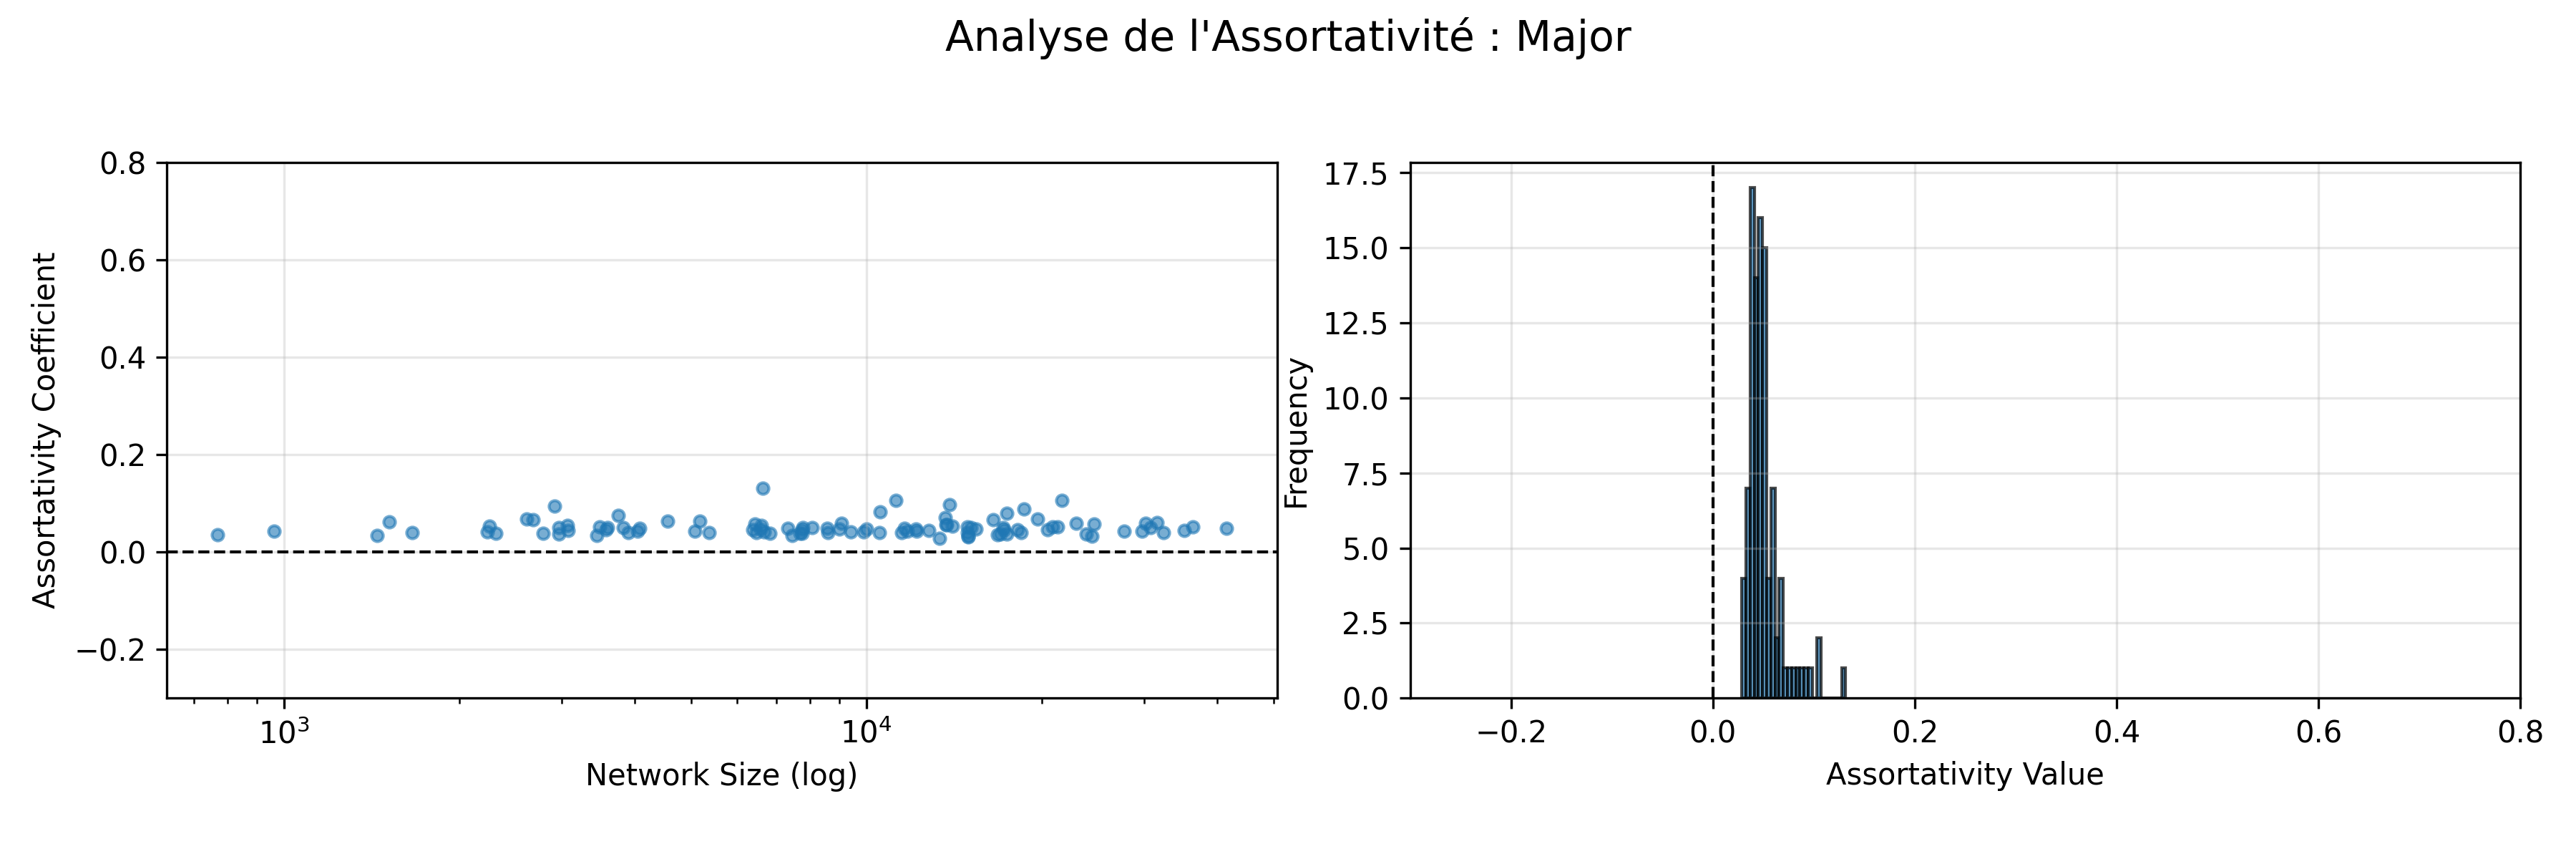
\includegraphics[width=0.9\textwidth]{q3_major.png}
    \caption{Analyse de l'assortativité pour la Spécialité (Major).}
    \label{fig:q3_major}
\end{figure}

\begin{figure}[H]
    \centering
    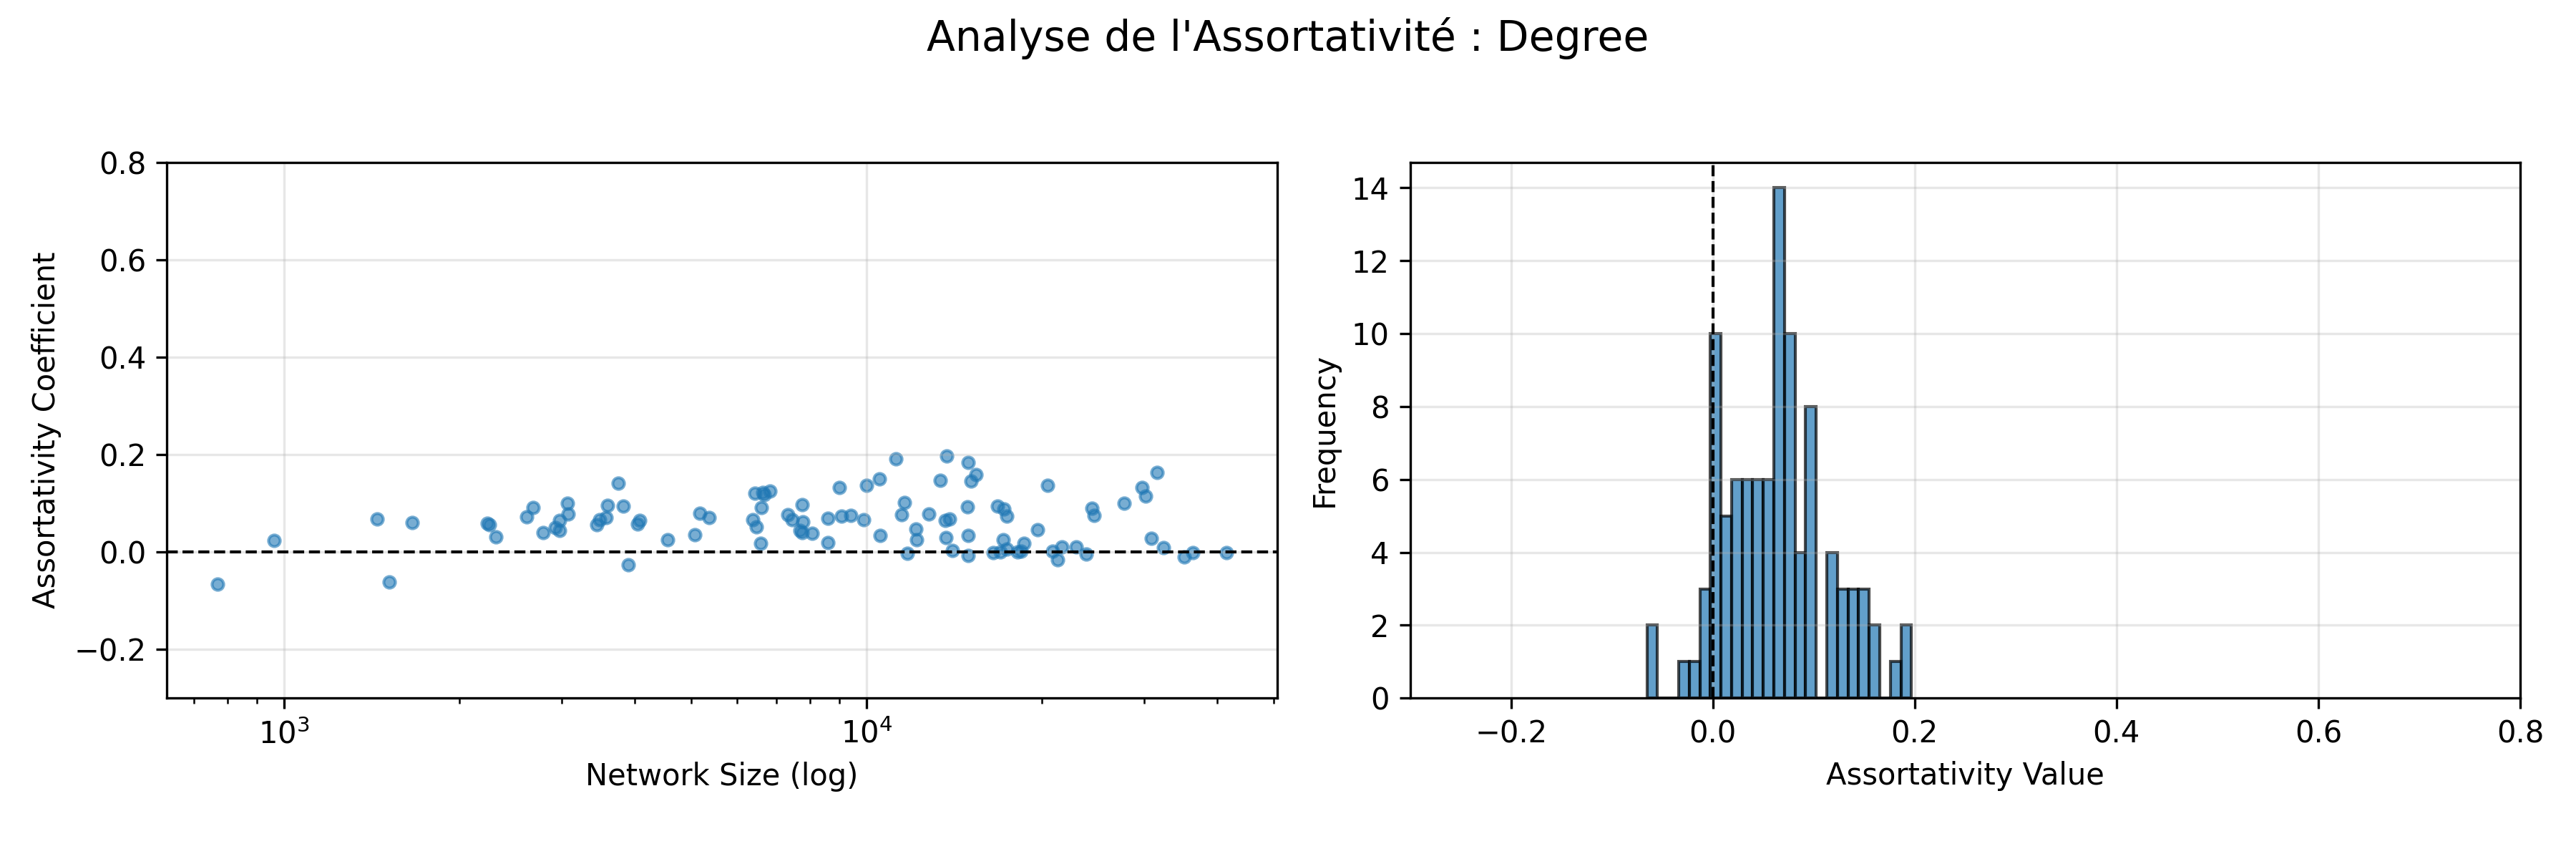
\includegraphics[width=0.9\textwidth]{q3_degree.png}
    \caption{Analyse de l'assortativité pour le Degré (Degree).}
    \label{fig:q3_degree}
\end{figure}

Pour la \textbf{Spécialité (Major)}, bien que la majorité des valeurs soient positives (autour de 0,1 à 0,2), la variance est plus prononcée. Travailler dans le même domaine d'études favorise les connexions (projets communs, mêmes classes), mais comme le soulignent certaines études, l'importance du "Major" dans la structure sociale varie de manière significative selon les institutions.

Concernant le \textbf{Degré}, la distribution est centrée autour de zéro, avec de nombreuses valeurs légèrement négatives. Cela indique que le réseau ne présente pas de stratification forte par popularité : les individus très connectés (les "hubs") ne sont pas uniquement amis avec d'autres hubs, mais se connectent à une grande variété d'étudiants, y compris ceux ayant peu d'amis.

\subsection{La dynamique de Genre (Assortativité quasi-nulle)}

\begin{figure}[H]
    \centering
    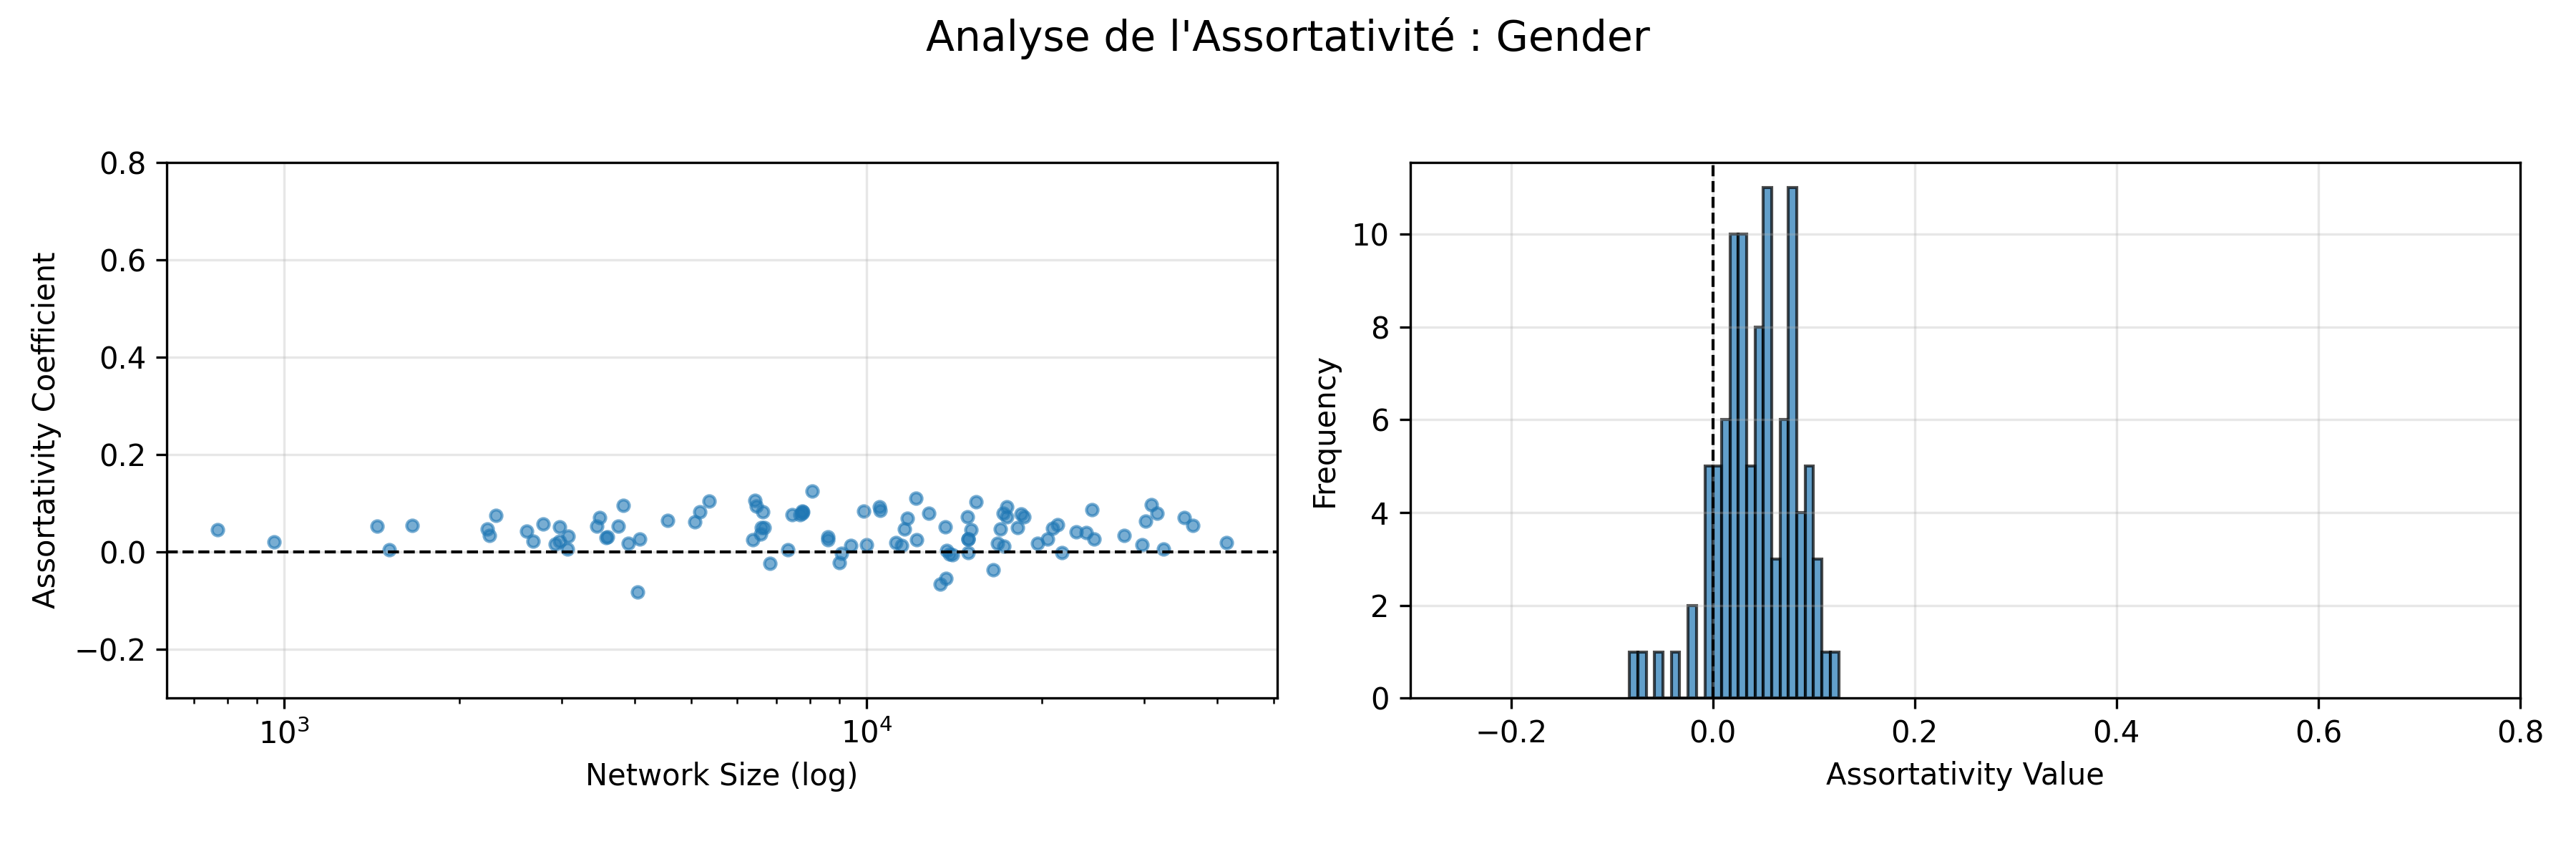
\includegraphics[width=0.9\textwidth]{q3_gender.png}
    \caption{Analyse de l'assortativité pour le Genre (Gender).}
    \label{fig:q3_gender}
\end{figure}

Comme attendu pour le \textbf{Genre}, la distribution des points s'étend de part et d'autre de la ligne d'assortativité nulle. Bien que la moyenne soit très légèrement positive (suggérant une infime tendance globale à s'associer avec le même genre), plusieurs réseaux affichent une assortativité négative (hétérophilie). Cette hétérophilie s'explique très probablement par la dynamique des relations amoureuses et des rencontres (hétéronormatives) au sein des campus.

\section{Question 4 : Prédiction de liens (Link Prediction)}

Cette section est dédiée à l'évaluation de la capacité de différents algorithmes à prédire l'apparition de liens d'amitié manquants. Afin d'évaluer la robustesse de nos approches à différentes échelles et face à la rareté des données, nous avons mené notre expérience sur deux réseaux distincts : Caltech (réseau de petite taille) et le MIT (réseau de grande taille). 

Pour répondre aux exigences d'une évaluation multicritère rigoureuse, nous avons aléatoirement supprimé différentes fractions $f \in [0.05, 0.1, 0.15, 0.2]$ des arêtes réelles pour constituer notre vérité terrain (\textit{Ground Truth}). Nous comparons trois prédicteurs topologiques classiques (Voisins Communs, Jaccard, Adamic/Adar) à une approche d'apprentissage profond : un Réseau de Neurones sur Graphes (GCN) muni d'une couche d'Embeddings apprenables.

\subsection{Évaluation quantitative selon la fraction d'arêtes supprimées}

Les tableaux ci-dessous résument la précision maximale (pour $k=400$ prédictions) obtenue par chaque méthode en fonction de la fraction $f$ d'arêtes supprimées.

\begin{table}[H]
    \centering
    \begin{tabular}{|l|c|c|c|c|}
        \hline
        \textbf{Méthode / Fraction $f$} & \textbf{0.05} & \textbf{0.10} & \textbf{0.15} & \textbf{0.20} \\
        \hline
        Common Neighbors & 0.2675 & 0.3975 & 0.5525 & 0.6475 \\
        Jaccard & 0.2300 & 0.3650 & 0.4475 & 0.4975 \\
        Adamic/Adar & 0.2700 & 0.4025 & 0.5675 & 0.6650 \\
        \textbf{GNN (GCN + Emb)} & \textbf{0.3425} & \textbf{0.5175} & \textbf{0.6800} & \textbf{0.7400} \\
        \hline
    \end{tabular}
    \caption{Précision@400 sur le réseau \textbf{Caltech} selon la fraction d'arêtes masquées.}
    \label{tab:q4_caltech}
\end{table}

\begin{table}[H]
    \centering
    \begin{tabular}{|l|c|c|c|c|}
        \hline
        \textbf{Méthode / Fraction $f$} & \textbf{0.05} & \textbf{0.10} & \textbf{0.15} & \textbf{0.20} \\
        \hline
        Common Neighbors & 0.4950 & 0.6525 & 0.7725 & 0.8300 \\
        Jaccard & 0.2525 & 0.3375 & 0.4050 & 0.4350 \\
        \textbf{Adamic/Adar} & \textbf{0.5175} & \textbf{0.6825} & \textbf{0.7900} & \textbf{0.8525} \\
        GNN (GCN + Emb) & 0.3525 & 0.4775 & 0.5575 & 0.6850 \\
        \hline
    \end{tabular}
    \caption{Précision@400 sur le réseau \textbf{MIT} selon la fraction d'arêtes masquées.}
    \label{tab:q4_mit}
\end{table}

\begin{figure}[H]
    \centering
    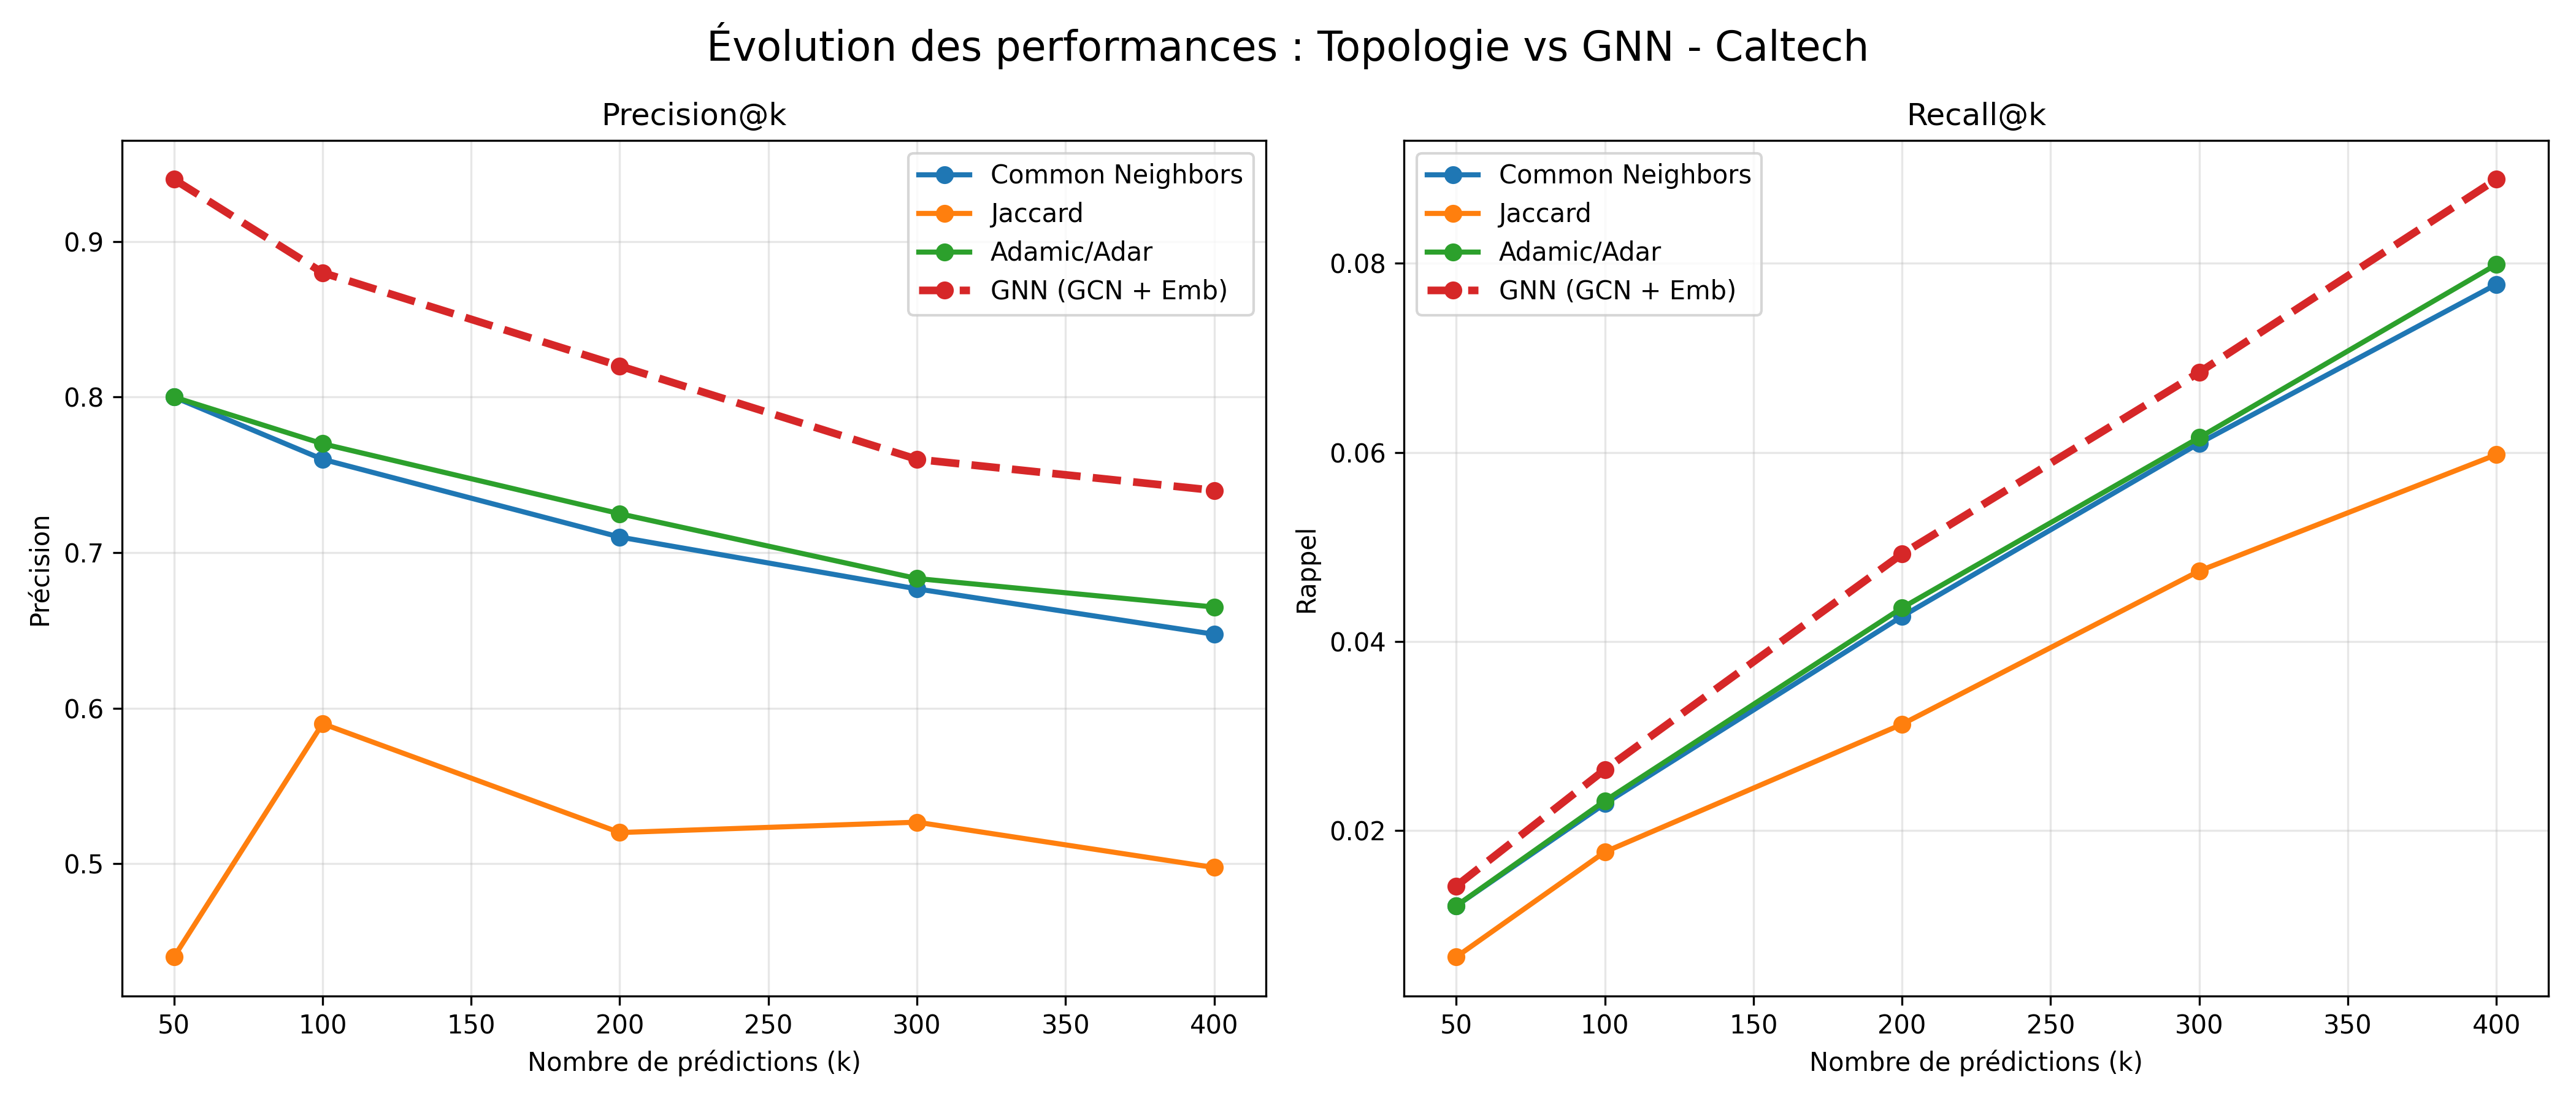
\includegraphics[width=0.9\textwidth]{q4caltech.png}
    \caption{Évolution de la prédiction de liens sur \textbf{Caltech} ($f=0.20$).}
    \label{fig:q4_caltech_plot}
\end{figure}

\begin{figure}[H]
    \centering
    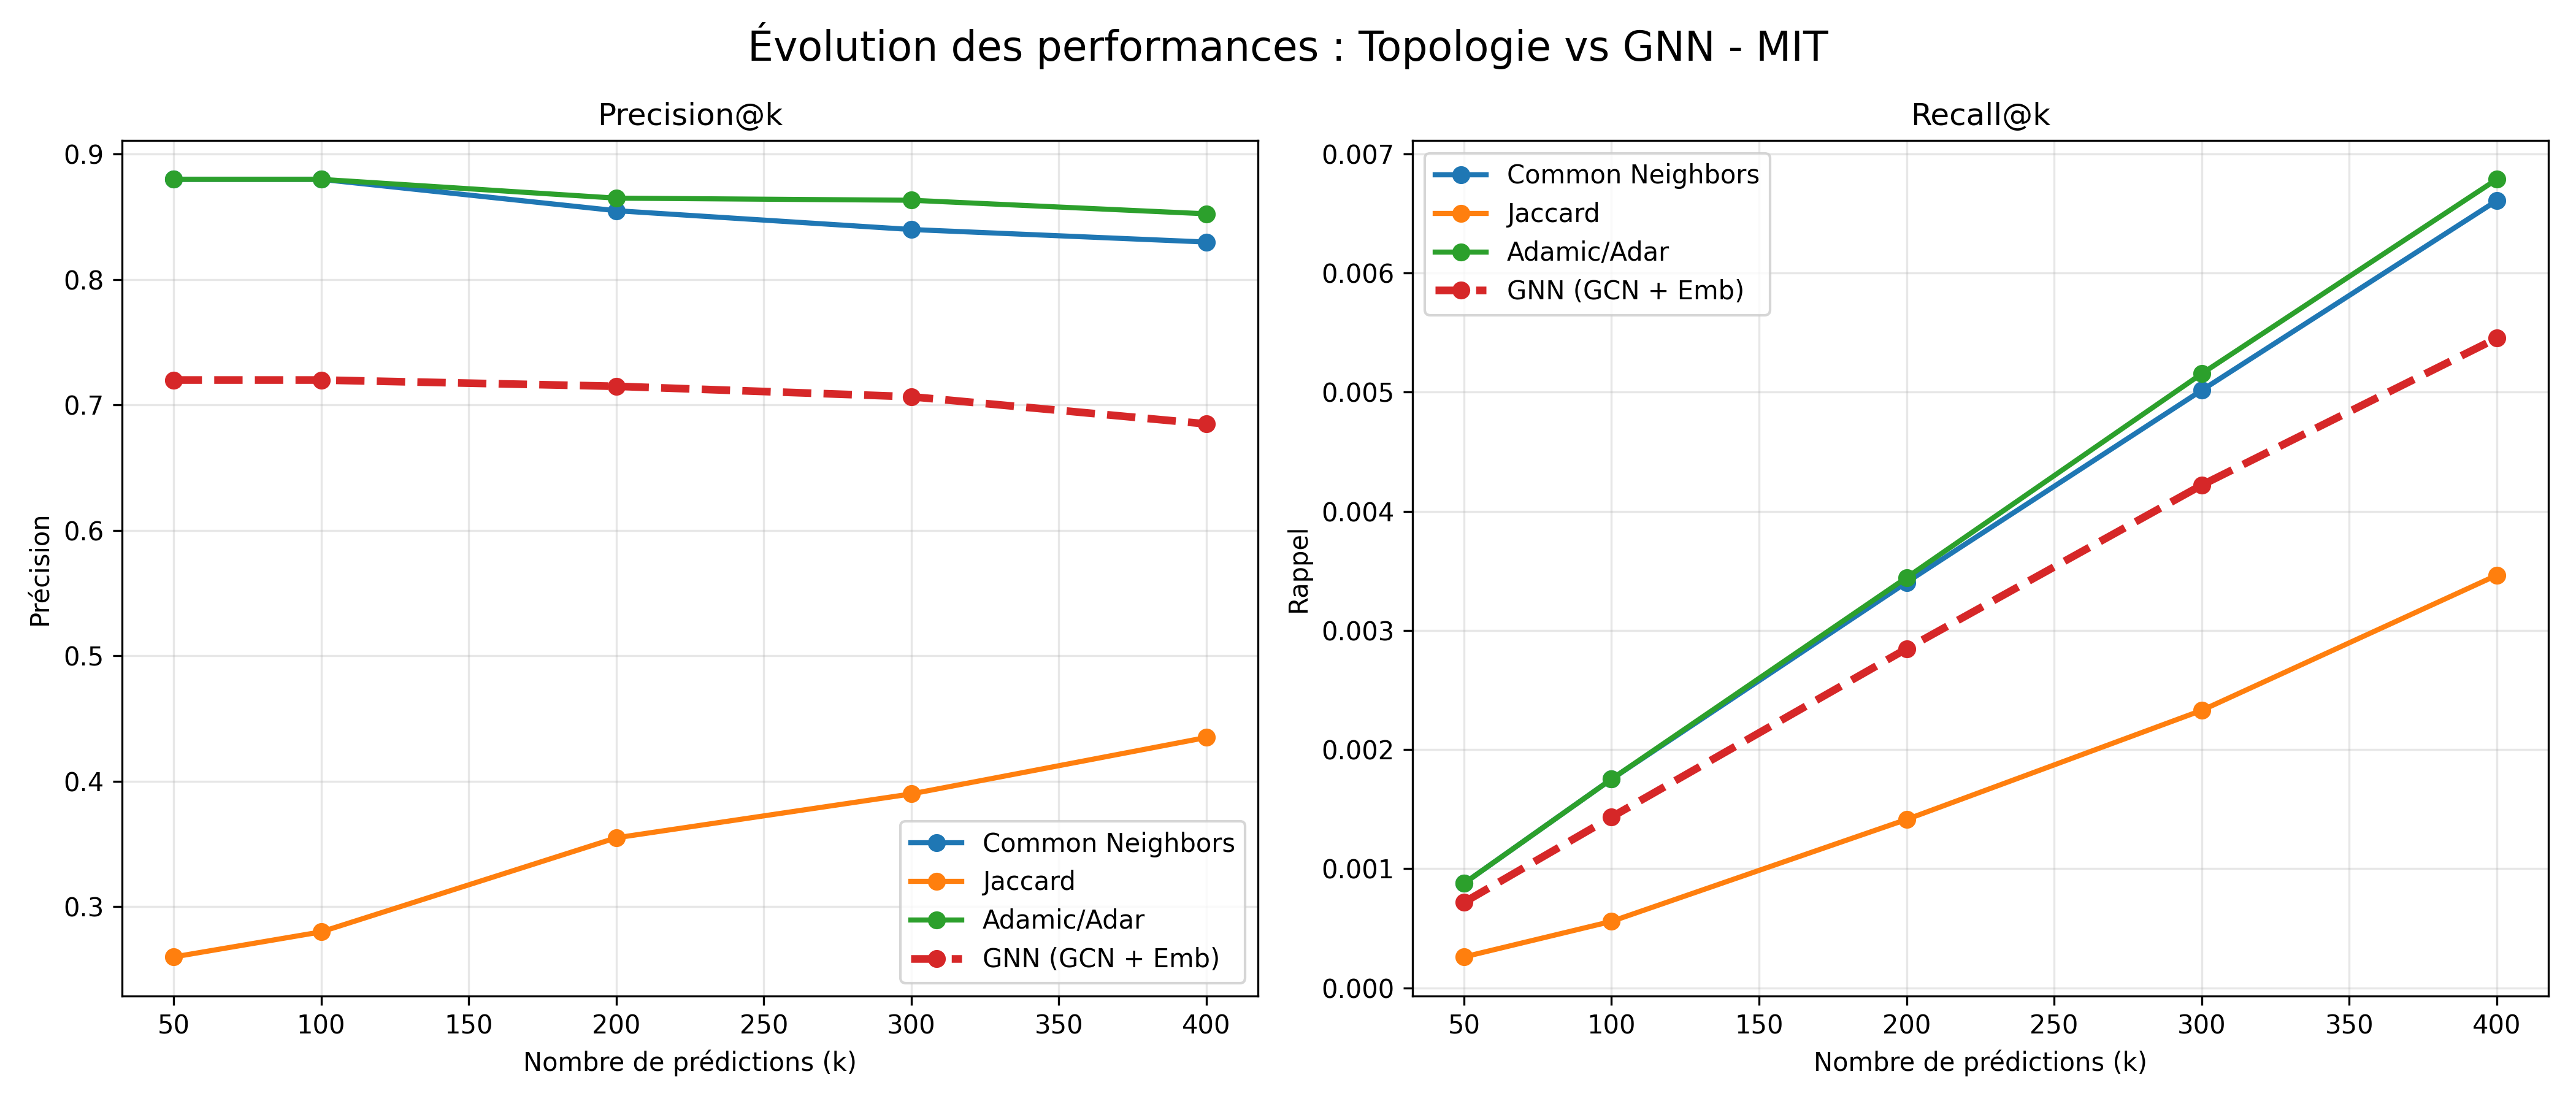
\includegraphics[width=0.9\textwidth]{q4mit.png}
    \caption{Évolution de la prédiction de liens sur le \textbf{MIT} ($f=0.20$).}
    \label{fig:q4_mit_plot}
\end{figure}

\subsection{Analyse des prédicteurs topologiques selon l'échelle}
L'introduction de multiples niveaux de rareté ($f$) confirme la solidité de la théorie des graphes. Sur le réseau de \textbf{Caltech}, les méthodes \textbf{Common Neighbors} et \textbf{Adamic/Adar} offrent des performances similaires à tous les niveaux de suppression. En revanche, sur le réseau vaste du \textbf{MIT}, \textbf{Adamic/Adar} se détache systématiquement et domine toutes les autres heuristiques, atteignant une précision remarquable de 85,25\% pour $f=0.2$.

Ce comportement est attendu : dans un réseau étendu, partager un ami commun qui est un "hub" (très populaire) n'a que peu de valeur prédictive. La pondération logarithmique inverse d'Adamic/Adar, qui pénalise ces hubs, s'avère redoutable. Le coefficient de Jaccard reste quant à lui le moins performant dans toutes les configurations, pénalisant de manière excessive l'union des voisinages.

\subsection{Limites du Deep Learning (GNN) face au passage à l'échelle}
Les résultats de notre modèle GCN offrent une excellente perspective sur la scalabilité des architectures d'apprentissage profond. Sur \textbf{Caltech}, le \textbf{GNN} réussit brillamment à surpasser les heuristiques topologiques, et ce, quelle que soit la fraction d'arêtes supprimées (jusqu'à 74\% de précision pour $f=0.2$). Il parvient à modéliser des représentations vectorielles efficaces pour ce nombre restreint de nœuds.

Cependant, sur le \textbf{MIT}, la performance du GNN s'effondre face aux heuristiques de base, se classant systématiquement derrière Adamic/Adar et Common Neighbors. Cette chute spectaculaire s'explique par la complexité du problème d'optimisation : devoir apprendre des embeddings \textit{ex nihilo} pour plus de 6400 nœuds — en l'absence totale d'attributs initiaux — nécessite un temps d'entraînement exponentiellement plus long et des ressources considérables. Cette limite démontre qu'en l'absence de \textit{features} riches, une heuristique topologique mathématiquement fondée s'avère beaucoup plus robuste, rapide et scalable qu'un réseau de neurones basique.

\section{Question 5 : Label Propagation (Classification de Nœuds)}

L'objectif de cette ultime section est d'inférer des attributs manquants (résidence, spécialité, genre) en s'appuyant sur la structure topologique du réseau, une tâche de classification semi-supervisée évaluée par l'exactitude (\textit{Accuracy}) et l'erreur absolue moyenne (\textit{MAE}).

\subsection{Justification des choix d'architecture (Question 5.b)}
Pour cette tâche, nous nous sommes inspirés des travaux de Kipf et Welling (2016) sur les Réseaux de Neurones Convolutifs sur Graphes (GCN). Notre architecture se justifie par :
\begin{itemize}
    \item \textbf{Embeddings apprenables :} En l'absence de caractéristiques initiales sur les nœuds, une couche \texttt{torch.nn.Embedding} permet au modèle d'apprendre une représentation vectorielle de la position topologique de chaque étudiant.
    \item \textbf{Profondeur et Régularisation :} Deux couches de convolution (\texttt{GCNConv}) permettent d'agréger l'information du voisinage. Nous utilisons un \textit{Dropout} ($p=0.5$) et une régularisation L2 ($5\times10^{-4}$) pour garantir la généralisation du modèle malgré le faible nombre de labels connus.
\end{itemize}

\subsection{Évaluation quantitative : Accuracy et MAE (Questions 5.c et 5.d)}
Conformément aux consignes, nous présentons ci-dessous les performances de l'algorithme pour différents taux de masquage ($10\%$, $20\%$ et $30\%$). L'évaluation de la MAE permet de mesurer la "distance" statistique de l'erreur, particulièrement pertinente pour des attributs à catégories multiples.

\begin{table}[H]
    \centering
    \small
    \begin{tabular}{|l|cc|cc|cc|}
        \hline
        \textbf{Caltech} & \multicolumn{2}{c|}{\textbf{10\% Masqués}} & \multicolumn{2}{c|}{\textbf{20\% Masqués}} & \multicolumn{2}{c|}{\textbf{30\% Masqués}} \\
        \hline
        \textbf{Attribut} & \textbf{Acc} & \textbf{MAE} & \textbf{Acc} & \textbf{MAE} & \textbf{Acc} & \textbf{MAE} \\
        \hline
        Dorm & 91.11\% & 0.2222 & 87.11\% & 0.3922 & 87.34\% & 0.4153 \\
        Major Index & 22.22\% & 7.7488 & 21.26\% & 8.3841 & 20.93\% & 8.6651 \\
        Gender & 76.19\% & 0.2381 & 72.86\% & 0.2714 & 73.49\% & 0.2651 \\
        \hline
    \end{tabular}
    \caption{Performances de classification sur \textbf{Caltech} (Accuracy et Mean Absolute Error).}
    \label{tab:q5_caltech}
\end{table}

\begin{table}[H]
    \centering
    \small
    \begin{tabular}{|l|cc|cc|cc|}
        \hline
        \textbf{MIT} & \multicolumn{2}{c|}{\textbf{10\% Masqués}} & \multicolumn{2}{c|}{\textbf{20\% Masqués}} & \multicolumn{2}{c|}{\textbf{30\% Masqués}} \\
        \hline
        \textbf{Attribut} & \textbf{Acc} & \textbf{MAE} & \textbf{Acc} & \textbf{MAE} & \textbf{Acc} & \textbf{MAE} \\
        \hline
        Dorm & 68.78\% & 6.3504 & 67.69\% & 6.5106 & 67.08\% & 6.7441 \\
        Major Index & 31.67\% & 5.2743 & 31.18\% & 5.4946 & 31.75\% & 5.4436 \\
        Gender & 80.46\% & 0.1954 & 80.98\% & 0.1902 & 80.65\% & 0.1935 \\
        \hline
    \end{tabular}
    \caption{Performances de classification sur le \textbf{MIT} (Accuracy et Mean Absolute Error).}
    \label{tab:q5_mit}
\end{table}

\begin{figure}[H]
    \centering
    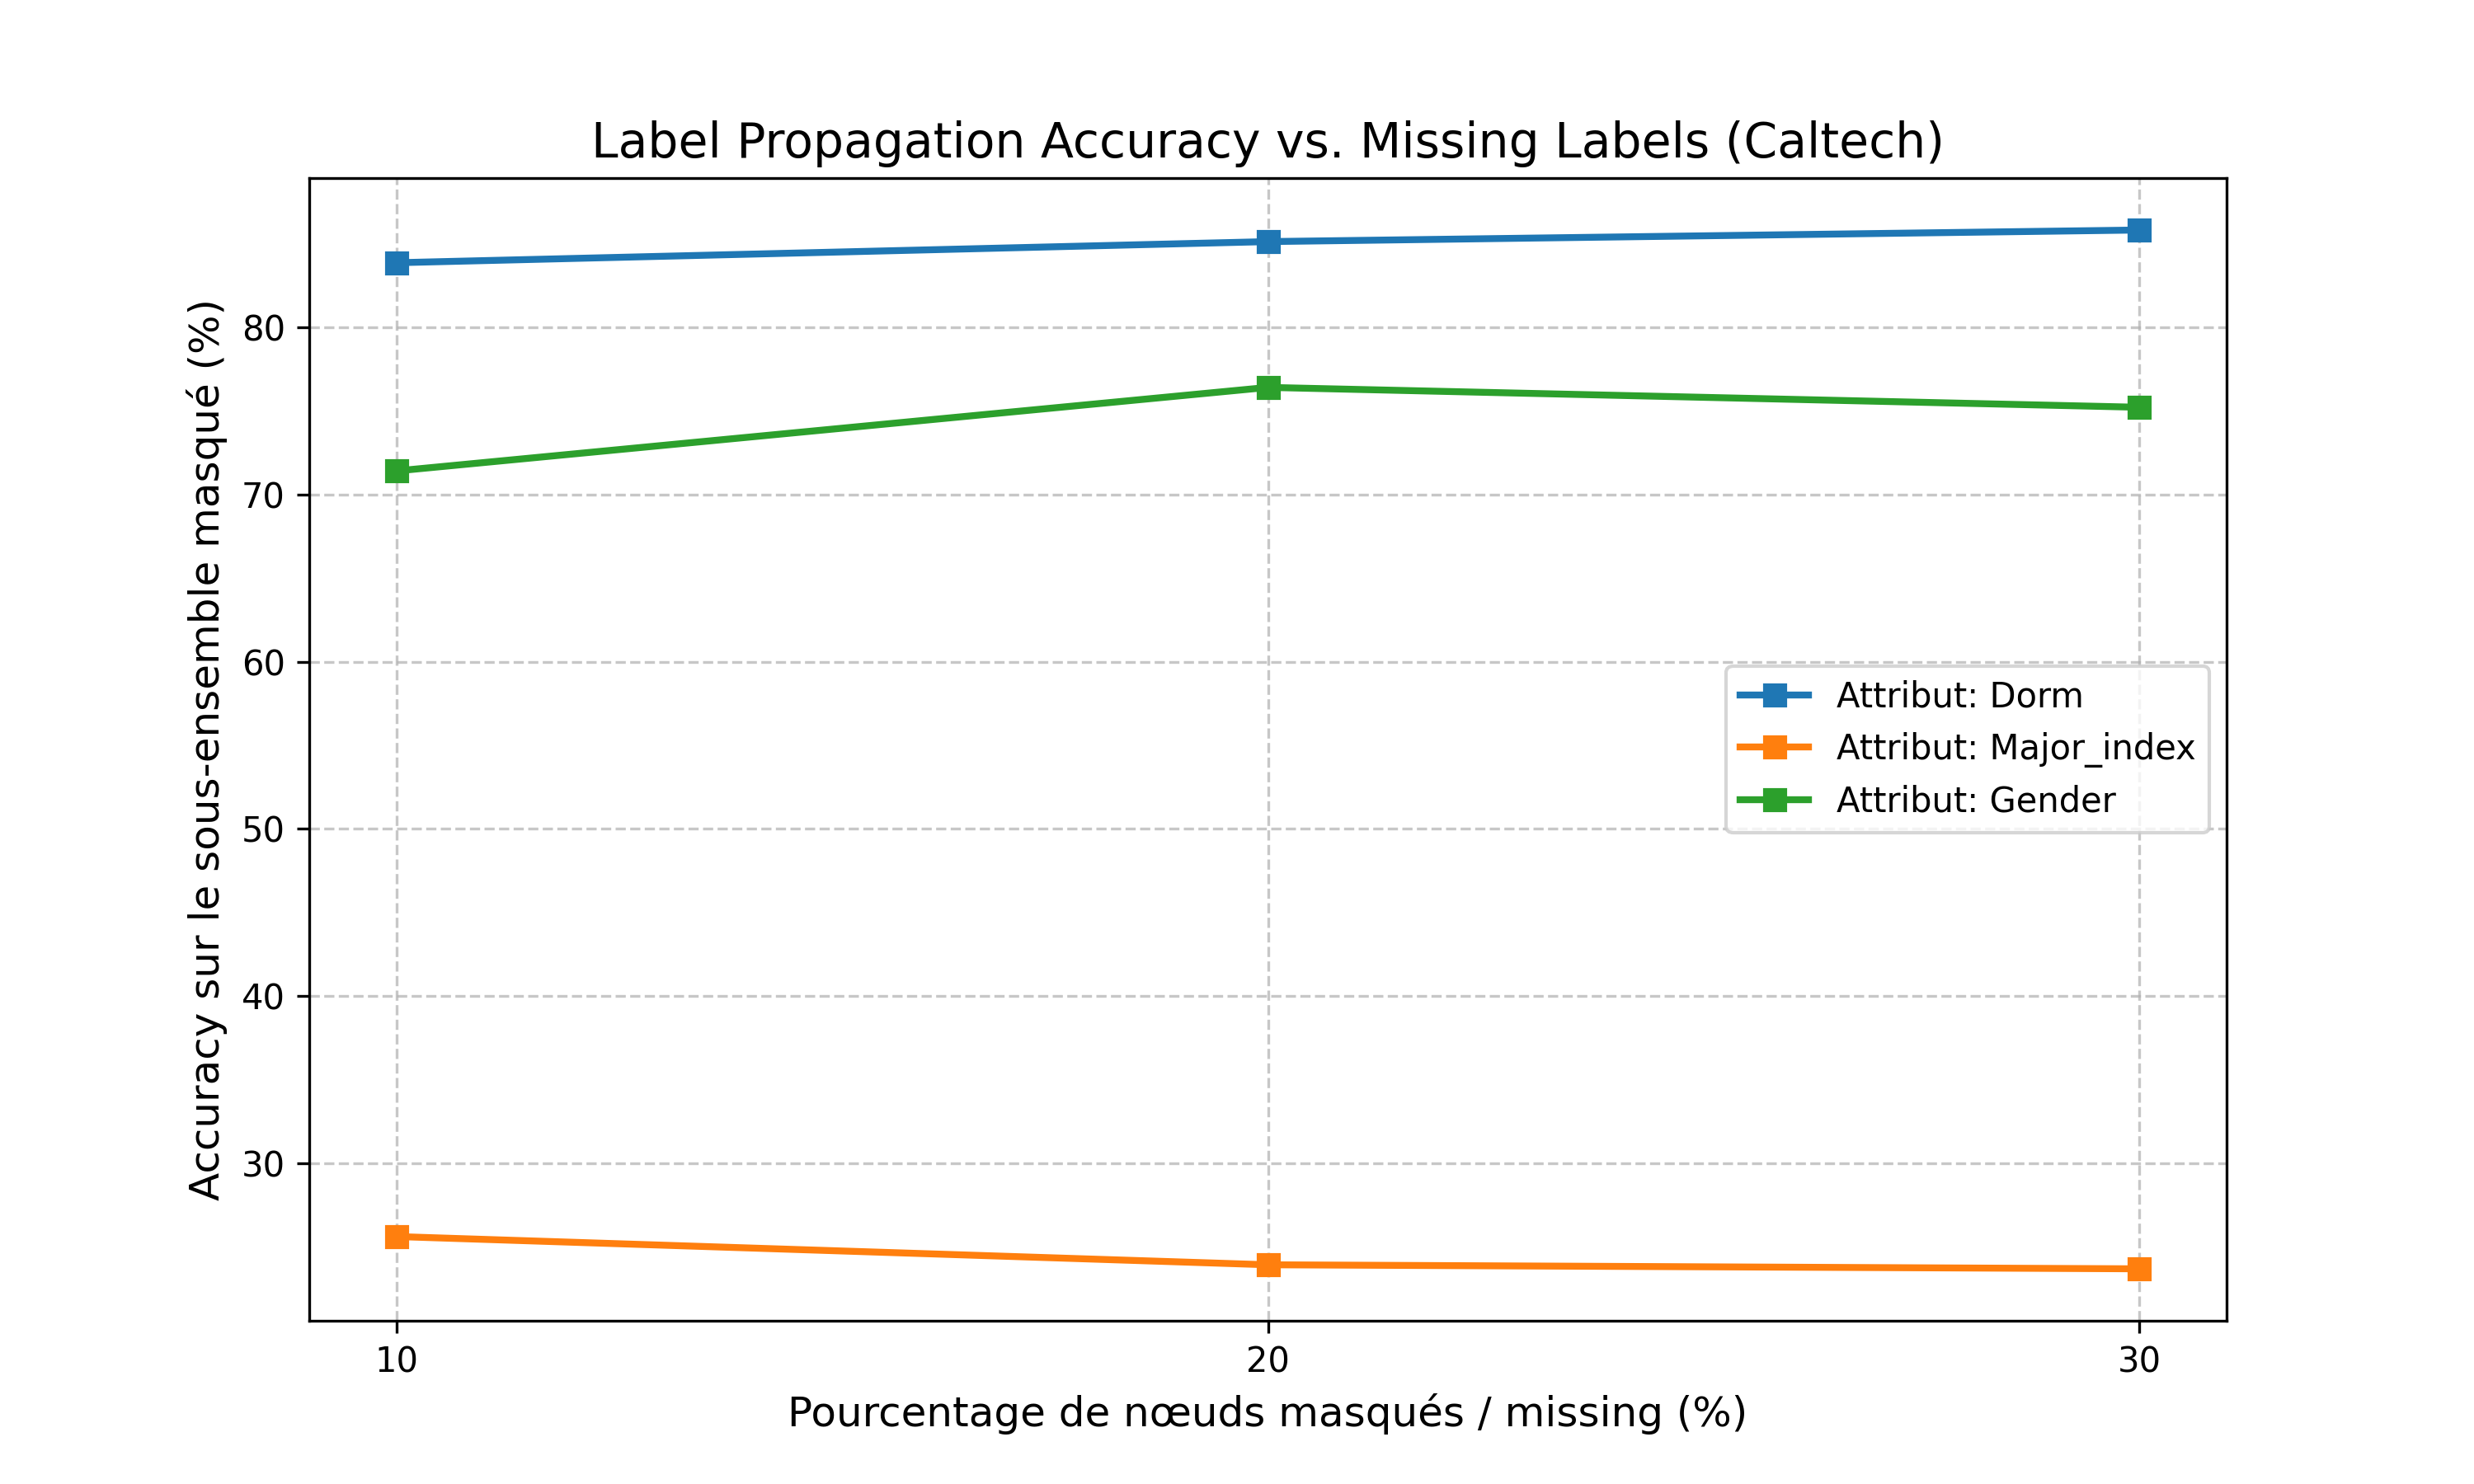
\includegraphics[width=0.85\textwidth]{q5_caltech_label_prop.png}
    \caption{Accuracy en fonction du masquage sur \textbf{Caltech}.}
    \label{fig:q5_caltech_plot}
\end{figure}

\subsection{Analyse et corrélations structurelles (Question 5.e)}
L'intégration de la MAE apporte un éclairage crucial sur la qualité de la propagation :

\begin{enumerate}
    \item \textbf{Dorm (Signal Spatial Fort) :} Sur Caltech, la MAE est extrêmement faible ($<0.5$), indiquant que même en cas d'erreur, le modèle prédit une catégorie très proche de la réalité. Cela confirme l'homophilie spatiale massive identifiée à la Q3. Au MIT, la MAE plus élevée (6.3 - 6.7) reflète la complexité d'un campus beaucoup plus vaste où la topologie est plus diffuse.
    \item \textbf{Major (Complexité Catégorielle) :} La spécialité présente les MAE les plus hautes (jusqu'à 8.6 sur Caltech). Cela démontre que l'erreur n'est pas "proche" : rater la spécialité d'un étudiant revient souvent à lui attribuer une majeure totalement différente, ce qui est cohérent avec la diversité des parcours académiques.
    \item \textbf{Gender (Biais et Robustesse) :} Le genre affiche une MAE très basse ($<0.2$) et une Accuracy stable autour de 80\%. Comme analysé précédemment, ce score élevé est en partie dû au déséquilibre démographique des réseaux (majorité masculine), le modèle minimisant l'erreur absolue en prédisant la classe majoritaire.
\end{enumerate}

En conclusion, la stabilité des scores entre 10\% et 30\% de masquage démontre la robustesse de l'architecture GCN pour capturer les régularités structurelles des réseaux sociaux universitaires, même avec une information parcellaire.

\section{Question 6 : Détection de Communautés (Community Detection)}

\subsection{Question de recherche et Hypothèse (6.a)}
\textbf{Question de recherche :} L'application d'un algorithme purement topologique de détection de communautés permet-elle de retrouver naturellement les divisions démographiques et institutionnelles d'une université ? 

\textbf{Hypothèse :} En nous basant sur nos découvertes de la Question 3 (fortes assortativités) et sur les travaux de Traud \textit{et al.} \cite{Traud2011, Traud2012}, nous postulons que la topologie du graphe est fortement conditionnée par les lieux de sociabilisation hors-ligne. Ainsi, un algorithme aveugle (ignorant les attributs) regroupera les nœuds en communautés qui se superposeront presque parfaitement avec l'attribut le plus assortatif du réseau (le dortoir pour Caltech, et un mix dortoir/année pour des réseaux plus vastes), mais échouera à segmenter le graphe selon des attributs non-assortatifs comme le genre.

\subsection{Validation expérimentale (6.b)}
Pour valider cette hypothèse, nous avons appliqué l'algorithme de \textbf{Louvain} (basé sur la maximisation de la modularité) sur les graphes de Caltech et du MIT. Pour mesurer mathématiquement la similarité entre les communautés détectées et les groupes réels (partitions basées sur les attributs), nous utilisons le score \textbf{NMI (Normalized Mutual Information)}. Le NMI varie de 0 (partitions indépendantes) à 1 (correspondance parfaite).

\begin{figure}[H]
    \centering
    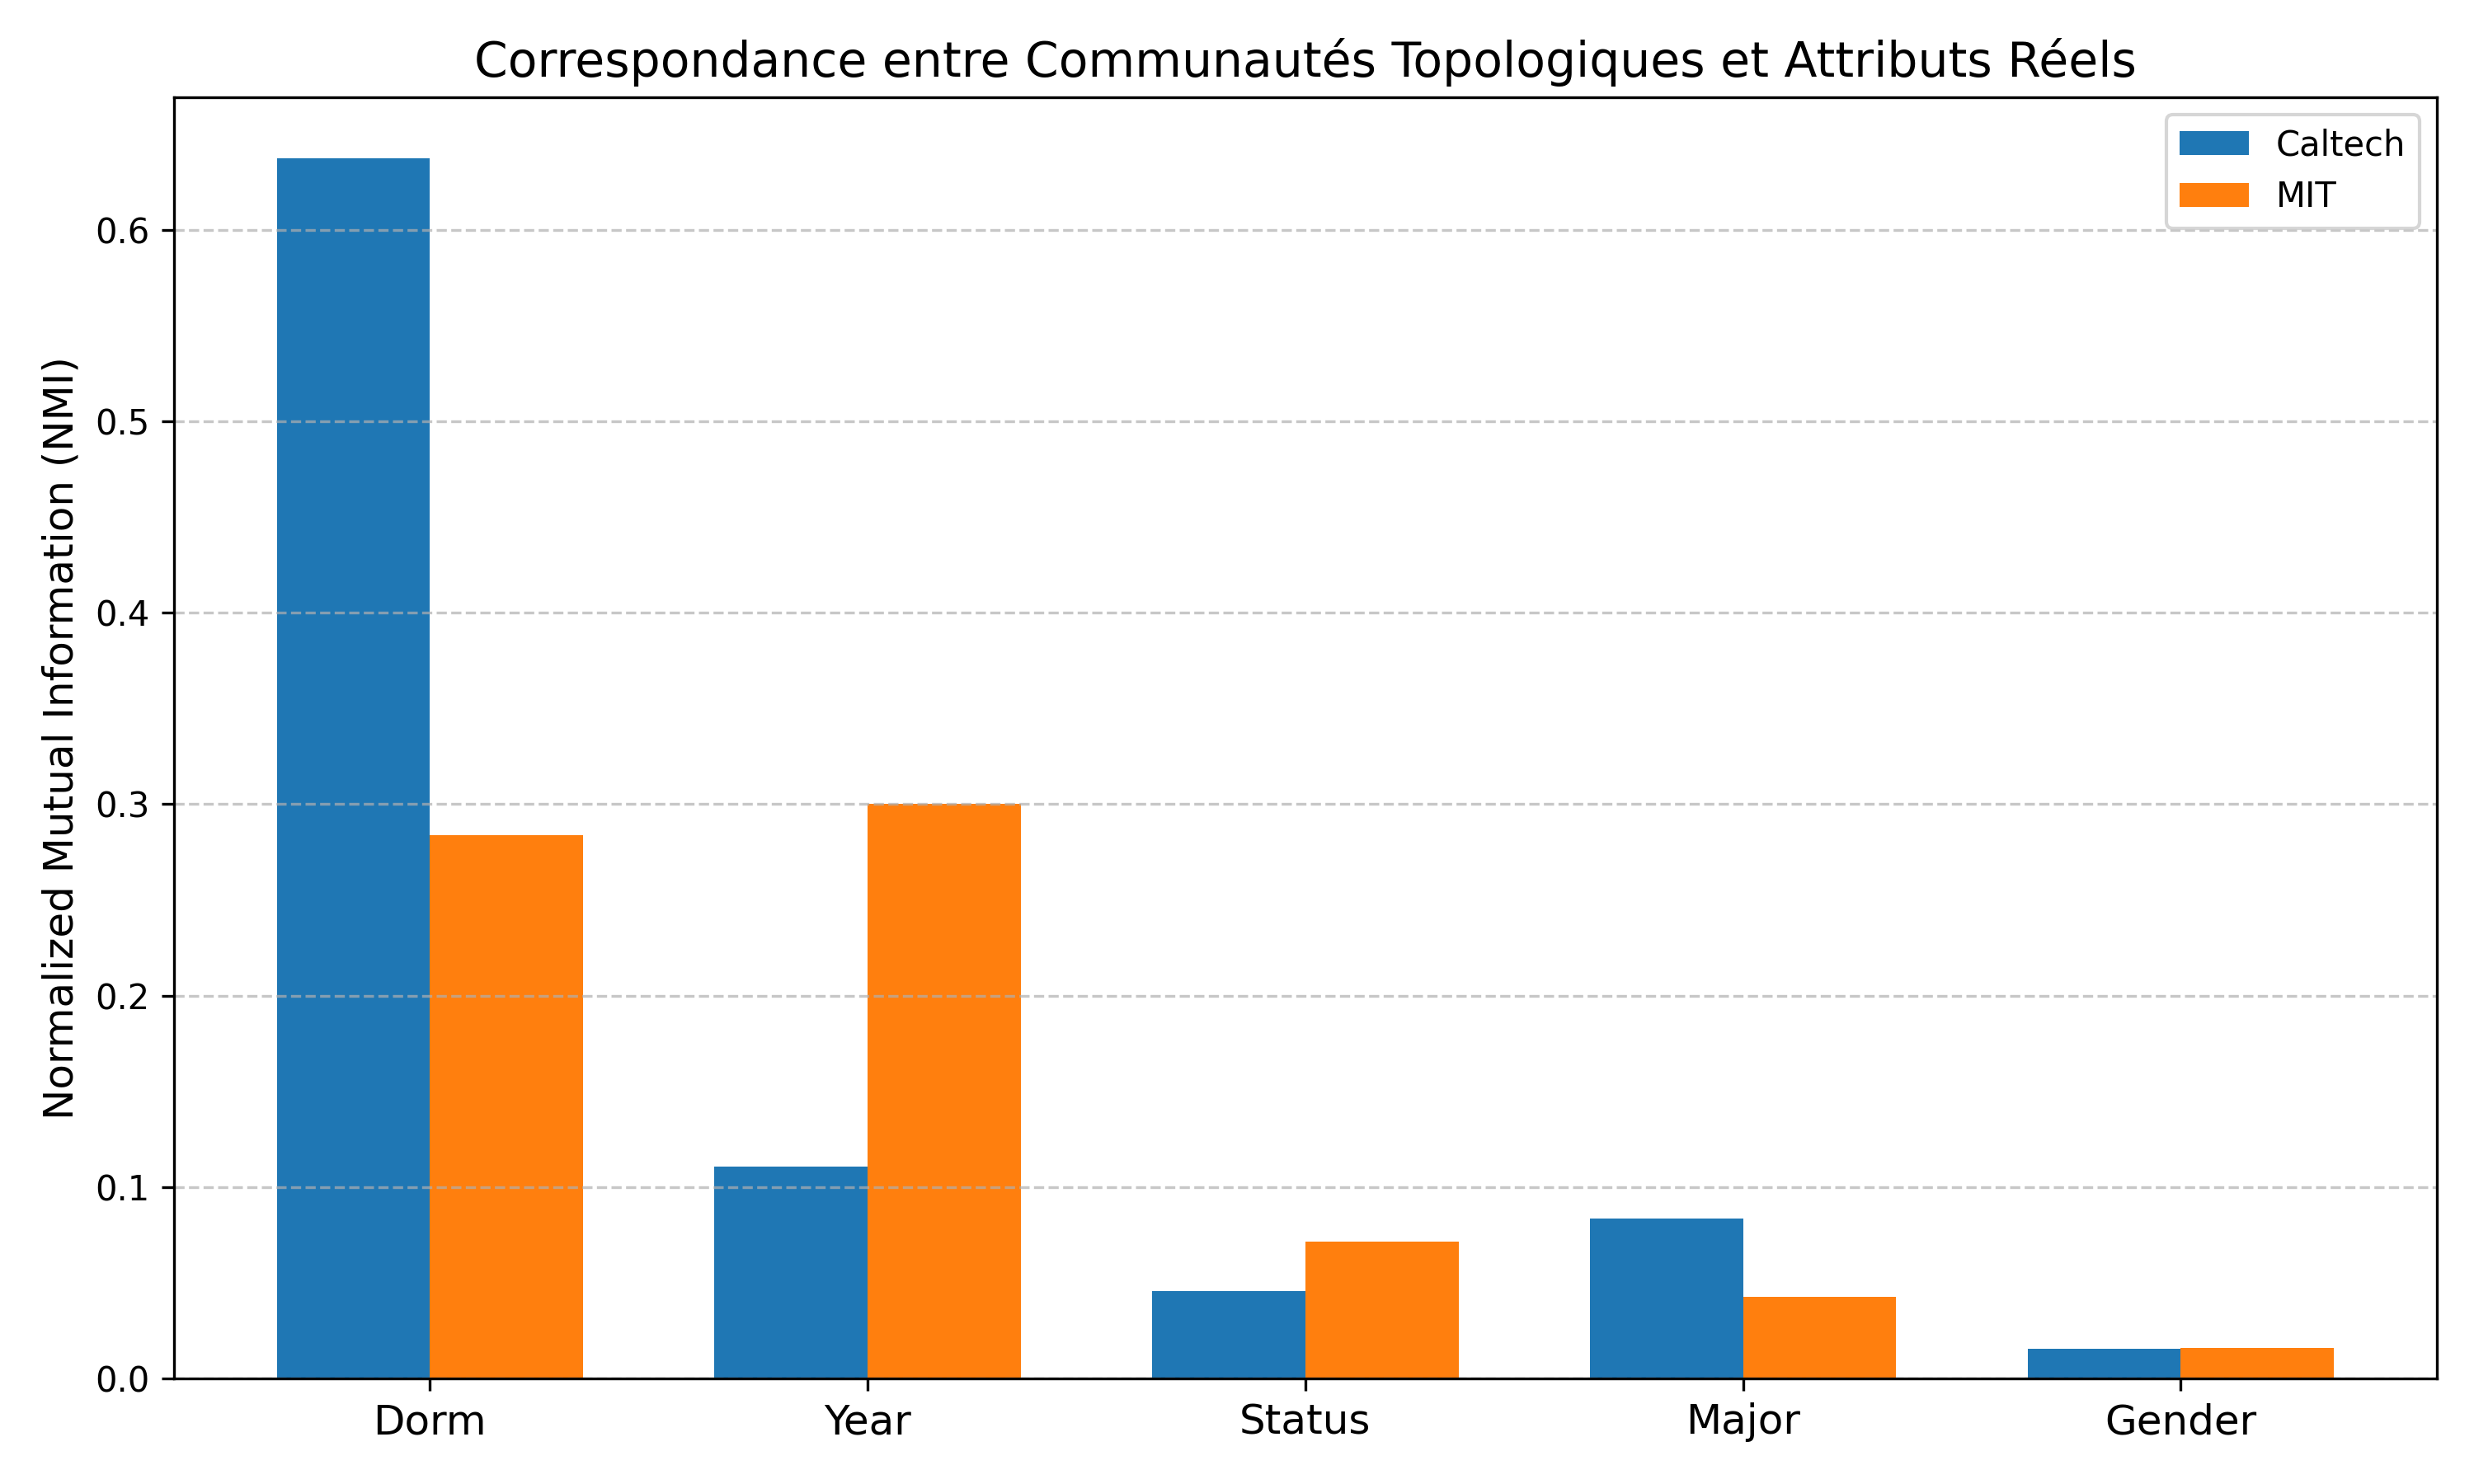
\includegraphics[width=0.85\textwidth]{q6_communities_nmi.png}
    \caption{Score NMI évaluant la correspondance entre les communautés topologiques (Louvain) et les véritables attributs des étudiants.}
    \label{fig:q6}
\end{figure}

\subsection{Analyse des résultats et Conclusion (6.c)}
L'exécution de l'algorithme et l'analyse de la Figure~\ref{fig:q6} valident notre hypothèse avec une précision remarquable :

\begin{enumerate}
    \item \textbf{L'empreinte topologique des dortoirs à Caltech :} L'algorithme a extrait \textbf{9 communautés} distinctes à Caltech. De manière frappante, le score NMI pour l'attribut \textbf{Dorm} atteint \textbf{0.6762}, écrasant tous les autres attributs. Sachant que le campus de Caltech s'articule historiquement autour d'un système très fermé de 8 \textit{Houses} (résidences), cela démontre que l'algorithme a pu virtuellement redessiner la carte du campus en observant uniquement les arêtes du réseau.
    \item \textbf{L'évolution avec l'échelle (MIT) :} Sur le réseau beaucoup plus vaste du MIT (6400 nœuds), l'algorithme a isolé \textbf{11 communautés}. La structure s'avère plus complexe : le \textbf{Dorm} reste dominant (NMI = 0.3124), mais l'année de promotion (\textbf{Year}) devient un critère de partitionnement majeur (NMI = 0.2769). Dans une grande université, la structure sociale se fracture donc de manière bimodale : les cercles d'amis se forment à l'intersection du lieu de vie et de la génération (camarades de promotion).
    \item \textbf{L'absence de ségrégation par le genre :} Le NMI pour l'attribut \textbf{Gender} est virtuellement nul sur les deux campus (\textbf{0.015} à Caltech et \textbf{0.009} au MIT). La détection de communautés prouve définitivement que le genre ne crée aucune fracture structurelle dans l'organisation de ces réseaux. La spécialité (\textbf{Major}), avec des scores NMI sous la barre des 0.10, s'avère également être un critère secondaire dans la formation des macro-communautés.
\end{enumerate}

\textbf{Conclusion finale :} Notre expérience confirme notre hypothèse. Les algorithmes de détection de communautés agissent comme de puissants "révélateurs" sociologiques. La structure d'un réseau en ligne comme \textit{Facebook100} n'est pas aléatoire : sa topologie est le calque numérique exact de l'organisation physique, logistique et institutionnelle des campus de la vie réelle.

% --- Bibliographie ---
\begin{thebibliography}{9}
\bibitem{Jacobs2015} Jacobs, A. Z., Way, S. F., Ugander, J. \& Clauset, A. (2015). Assembling thefacebook. \textit{WebSci '15}. 
\bibitem{Traud2011} Traud, A. L., Kelsic, E. D., Mucha, P. J. \& Porter, M. A. (2011). Comparing community structure to characteristics. \textit{SIAM Review}. 
\bibitem{Traud2012} Traud, A. L., Mucha, P. J. \& Porter, M. A. (2012). Social structure of facebook networks. \textit{Physica A}. 
\bibitem{Kipf2016} Kipf, T. N. \& Welling, M. (2016). Semi-supervised classification with graph convolutional networks. \textit{CoRR abs/1609.02907}.
\end{thebibliography}

\end{document}